\documentclass[10pt]{beamer}
\usepackage[utf8]{inputenc}

\usepackage{multirow,rotating}
\usepackage{color}
\usepackage{tikz-cd}
\usepackage{array}
\usepackage{siunitx}
\usepackage{mathtools,nccmath}%
\usepackage{etoolbox, xparse} 
\usepackage{amsfonts}
\usepackage{amssymb}
\usepackage{amsthm}
\usepackage{amsmath}
\usepackage{amsopn}
\usepackage{pifont}
\usepackage{xcolor}
\usepackage{booktabs}

\usepackage{float}

\usepackage{epstopdf}
\epstopdfDeclareGraphicsRule{.tif}{png}{.png}{convert #1 \OutputFile}
\AppendGraphicsExtensions{.tif}

\usetheme{CambridgeUS}
\usecolortheme{dolphin}
\makeatletter
\setbeamertemplate{footline}
{
  \leavevmode%
  \hbox{%
  \begin{beamercolorbox}[wd=.333333\paperwidth,ht=2.25ex,dp=1ex,center]{author in head/foot}%
    \usebeamerfont{author in head/foot}\insertshortauthor%~~\beamer@ifempty{\insertshortinstitute}{}{(\insertshortinstitute)}
  \end{beamercolorbox}%
  \begin{beamercolorbox}[wd=.333333\paperwidth,ht=2.25ex,dp=1ex,center]{title in head/foot}%
    \usebeamerfont{title in head/foot}\insertshorttitle
  \end{beamercolorbox}%
  \begin{beamercolorbox}[wd=.333333\paperwidth,ht=2.25ex,dp=1ex,right]{date in head/foot}%
    \usebeamerfont{date in head/foot}\insertshortdate{}\hspace*{2em}
    \insertframenumber{} / \inserttotalframenumber\hspace*{2ex} 
  \end{beamercolorbox}}%
  \vskip0pt%
}
\makeatother


\setbeamertemplate{caption}[numbered]


% set colors
\definecolor{myNewColorA}{RGB}{158, 27,50}
\definecolor{myNewColorB}{RGB}{158, 27,50}
\definecolor{myNewColorC}{RGB}{158, 27,50} % {130,138,143}
\setbeamercolor*{palette primary}{bg=myNewColorC}
\setbeamercolor*{palette secondary}{bg=myNewColorB, fg = white}
\setbeamercolor*{palette tertiary}{bg=myNewColorA, fg = white}
\setbeamercolor*{titlelike}{fg=myNewColorA}
\setbeamercolor*{title}{bg=myNewColorA, fg = white}
\setbeamercolor*{item}{fg=myNewColorA}
\setbeamercolor*{caption name}{fg=myNewColorA}
\setbeamercolor*{button}{bg=myNewColorA,fg= white}
\usefonttheme{professionalfonts}
\usepackage{natbib}

%------------------------------------------------------------
% \titlegraphic{\includegraphics[height=0.75cm]{ua_eng_logo.png}} 

% logo of my university


%\titlegraphic{%
%\includegraphics[width=3.0cm]{ua_seal.png}
%}

\setbeamerfont{title}{size=\large}
\setbeamerfont{subtitle}{size=\small}
%\setbeamerfont{author}{size=\small}
\setbeamerfont{date}{size=\footnotesize}
\setbeamerfont{institute}{size=\footnotesize}

%\date[\textcolor{white}{Conference Name, 2022}]
%{Conference full name\\
%Aug 29-30, 2022}

%------------------------------------------------------------
%This block of commands puts the table of contents at the 
%beginning of each section and highlights the current section:
%\AtBeginSection[]
%{
%  \begin{frame}
%    \frametitle{Contents}
%    \tableofcontents[currentsection]
%  \end{frame}
%}
%\AtBeginSection[]{
 % \begin{frame}
 % \vfill
  %\centering
  %\begin{beamercolorbox}[sep=8pt,center,shadow=true,rounded=true]{title}
    %\usebeamerfont{title}\insertsectionhead\par%
 % \end{beamercolorbox}
  %\vfill
  %\end{frame}

% ------Contents below---
%------------------------------------------------------------

\begin{document}
\author[I. Barriola, R. Chaba]{I. Barriola\inst{1} \and R. Chaba\inst{2}}

\institute{
	\inst{1} CRED, Paris Panthéon Assas University, Paris, France
	\and
	\inst{2} LEMMA, Paris Panthéon Assas University, Paris, France
}
\title{Internet and Nation Building in Africa}
\subtitle{Preliminary results}
\date{September 12, 2024}

\begin{frame}
    \titlepage
\end{frame}

    

\begin{frame}{Motivation}
%\centering\textbf{Nation building needs citizens involvement}\vspace{1em}
    \begin{itemize}\setlength\itemsep{1em}
        \item \textbf{Trust in national institutions} promotes state legitimacy, civic engagement, social cohesion
        \begin{itemize}
            \item Crucial concern in Africa since the post-colonial era
        \end{itemize}
        \item However, the \textbf{nature of trust} is key for expecting favorable outcomes
        \item  \textbf{High levels of trust in institutions can be misleading} if citizens are uninformed or uninterested\\ \vspace{1em}
        $\rightarrow{}$ Such \textbf{default trust} can disrupt accountability mechanisms, weakening the political power of citizens and their relationship with the nation        %\item Information on governance can be acquired through direct experience or communication networks
    \end{itemize}
\end{frame}





\begin{frame}{Motivation}
    \centering\textbf{Most African capitals lie in peripheral areas rather than central locations}\vspace{1em}
    \begin{itemize}\setlength\itemsep{1em}
        \item Large parts of the population live far from their capital city
        \item 80\% of African constitutions feature highly centralized states \textit{(Kuperman, 2015)}
        %\begin{itemize}
         %   \item  Ineffective accountability mechanisms reduce incentives for public investments in remote areas (e.g. McKay et al. 2023, Provenzano 2024)
        %\end{itemize}
        \item Institutions struggle to reach remote areas
        \begin{itemize}\vspace{0.5em}
            \item Lack of state presence in remote areas \textit{(Provenzano, 2024)}\vspace{0.5em}\\
            $\rightarrow{}$ Spatial disparities in state interaction

        \end{itemize}
    \end{itemize}
\end{frame}

\begin{frame}{Motivation}
        \begin{itemize}\vspace{0.5em}
            \item Information about governance can be obtained through \textbf{direct experience} or \textbf{communication networks}\vspace{0.5em}
            \item Remote populations:\\
            \begin{itemize}
            \item are less likely to directly encounter governance wrongdoing due to the \textbf{lack of state presence}\vspace{0.5em}
            \item consume news less frequently due to the \textbf{lack of access}\\ \vspace{1em}
            \end{itemize}
            $\rightarrow$ \definecolor{rougeprez}{RGB}{158,27,50}\textcolor{rougeprez}{\textbf{Remote populations are more prone to showing default trust in institutions}} 
         \end{itemize}

\end{frame}
\begin{frame}{Motivation}
    \centering\vspace{1em}
    \begin{itemize}\setlength\itemsep{1em}
    %\item Dysfunction of accountability mechanisms reduces incentives for public investments and nation building in remote areas
    \item \textbf{Access to new channels of information} about government activities can \textbf{reshape perceptions} of institutions in remote areas\\ \vspace{0.5em}
    $\rightarrow{}$ \textbf{Expanding internet access} can enhance information consumption and \textbf{reduce spatial disparities} in institutional trust
    \end{itemize}\vspace{3em}
    \centering \definecolor{rougeprez}{RGB}{158,27,50}\textcolor{rougeprez}{\textbf{Replace default trust with critical evaluation to restore accountability mechanisms needed for nation-building}}
\end{frame}

\begin{frame}{Research question}

\centering \textbf{How does the diffusion of mobile internet affect political accountability in remote areas?}
\vspace{15pt}
\begin{itemize}\setlength\itemsep{1em}
    \item Hypothesis:
    \vspace{10pt}
    \begin{itemize}
    \item \definecolor{rougeprez}{RGB}{158,27,50}\textcolor{rougeprez}{\textbf{H1}}: \textbf{Living in remote areas is associated with higher levels of institutional trust}
        \vspace{10pt}
    \item \definecolor{rougeprez}{RGB}{158,27,50}\textcolor{rougeprez}{\textbf{H2}}: \textbf{Expanding internet access mitigates spatial disparities in institutional trust}
    \end{itemize}
\end{itemize}
\end{frame}



\begin{frame}{Literature contribution}

\begin{itemize}\setlength\itemsep{1em}
    \item Institutional trust and nation building
    \begin{itemize}
        \item \textit{e.g. Aghion et al. (2010), Algan and Cahuc (2013), McKay et al. (2019)}\\
        $\rightarrow{}$ \textbf{High levels of trust can be misleading for nation building}
    \end{itemize}    
    \item Political economy of the capital city
\begin{itemize}
    \item \textit{e.g.  Mann (1993), Michalopoulos and Papaioannou (2014), Campante et al. (2019), Provenzano (2024)}\\
    $\rightarrow{}$ \textbf{Distance to the capital city shapes institutional perceptions}
\end{itemize}
\item Internet role in accountability and governance information
    \begin{itemize}
        \item \textit{e.g. Manacorda \& Tesei (2020), Guriev et al. (2021), Cariolle et al. (2024)}\\
        $\rightarrow{}$ \textbf{Expanding internet access can enhance accountability mechanisms}
    \end{itemize}
    
\end{itemize}
\end{frame}

\begin{frame}{Main Data}
\begin{columns}
\begin{column}{0.5\textwidth}
\begin{itemize}\setlength\itemsep{1em}
\item Afrobarometer surveys accross 20 Sub-Saharan countries: wave 5 to 7 (2011-2018)
\begin{itemize}
    \item Geolocated data, N $\approx$ 85 000
    \item Public attitude survey on democracy, governance, media consumption
    \item Construction of distance variables
    %\item Construction of normalized isolation measure (values between 0 and 1) \\
  % \[
%\frac{\text{distance from the capital city}}{\text{maximal distance from the capital city}}
%\]
\end{itemize}
\item Collins Bartholomew’s Mobile Coverage Explorer: 2G/3G network coverage (2011-2018)
\begin{itemize}
    \item 1×1-kilometer binary grid cells
    \item ADM2 level mean coverage
    \item Weighted by UN-adjusted population density grid
\end{itemize}
%\item Other sources for controls: V-DEM, World Bank, Africa Integrity Indicators...
\end{itemize}

\end{column}
\begin{column}{0.5\textwidth}

\begin{figure}
    \centering
    \caption{Respondents and capital cities}
    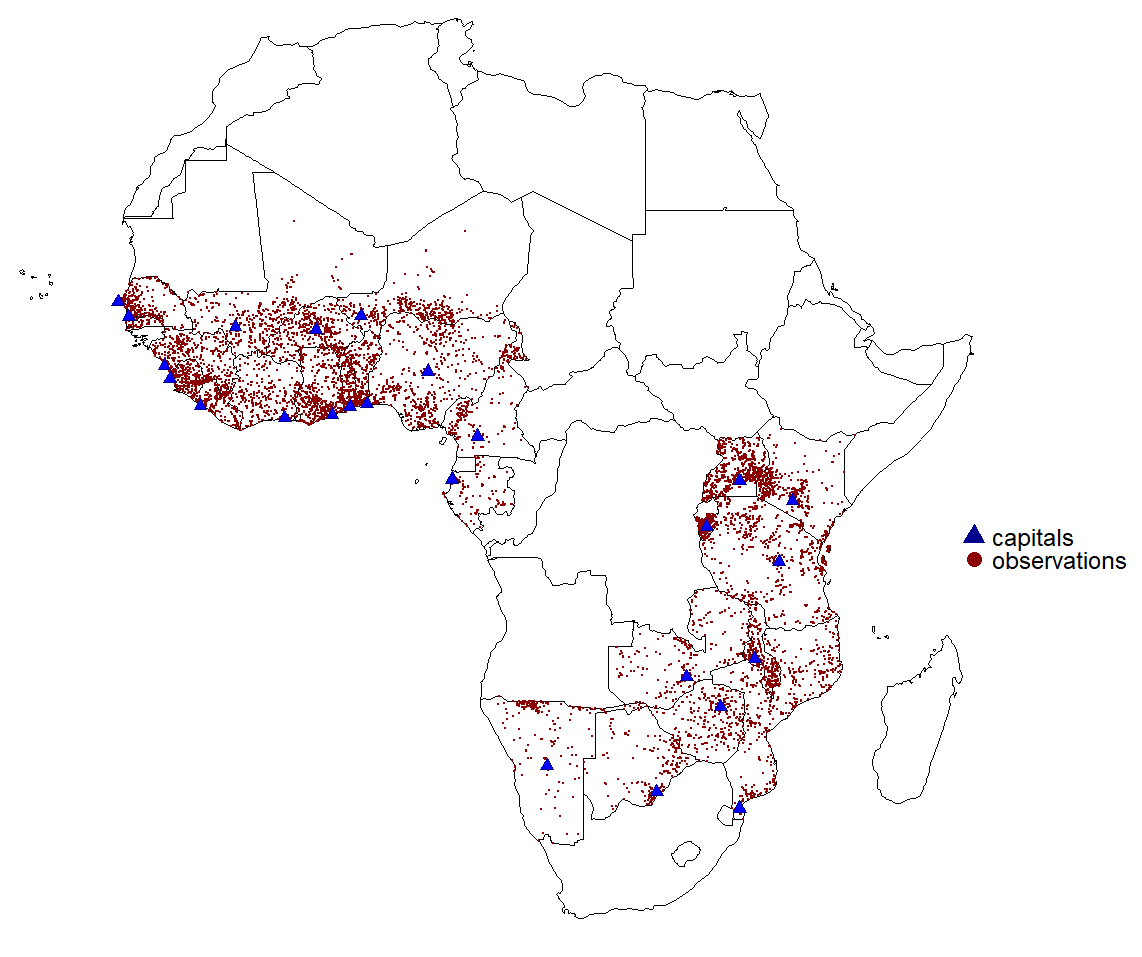
\includegraphics[width=6cm]{carte afrique echantillon total.png}
\end{figure}
\end{column}
    \end{columns}
    

\end{frame}
\begin{frame}{Empirical Strategy - Distance on institutional trust (1)}
    \centering \textbf{Effect of distance to the capital city on institutional trust}\vspace{1em}
    \begin{itemize}
        \item OLS
        \begin{equation}
        trust_{ict} = \beta_{0} + \beta_{1}distance_{ict} + BX_{i} + \mu_{ct} + \varepsilon_{ict}
        \end{equation}
        \begin{itemize}
            \item $trust_{ict}$ : mean of trust measures in parliament, president and electoral commission (values between 0 and 3)\vfill
            \item $distance_{ict}$ : normalized distance measure (values between 0 and 1)\\
            $\rightarrow{}$ \textit{e.g. Michalopoulos and Papaioannou (2014)}\vfill
            \item $X_i$ : set of individual controls\vfill
            \item $\mu_{ct}$ : country $\times$ round fixed effects\vfill
            \item $\epsilon_{ict}$ : error term\vfill
            \item Robust standard errors clustered at the ADM2 x round level
        \end{itemize}
    \end{itemize}
\end{frame}



\begin{frame}{Empirical Strategy - Distance on institutional trust (2)}
    \begin{itemize}
        \item Border discontinuity design
\begin{columns}
\begin{column}{0.5\textwidth}
\begin{itemize}
    \item Similar identification strategy as \textit{Michalopoulos and Papaioannou (2014), de Figueiredo et al. (2023), Provenzano (2024)}\vspace{0.3cm}
    \item We use Murdock's (1959) historical ethnic homeland map and assume that post-colonial African borders were established independently of ethnic regions\vspace{0.3cm}
    \item \textbf{Main assumption:} Two individuals living in the same historical ethnic region share similar unobserved characteristics
\end{itemize}
\end{column}

\begin{column}{0.5\textwidth}
\begin{figure}
    \centering
    \caption{Historical ethnic homeland map}
    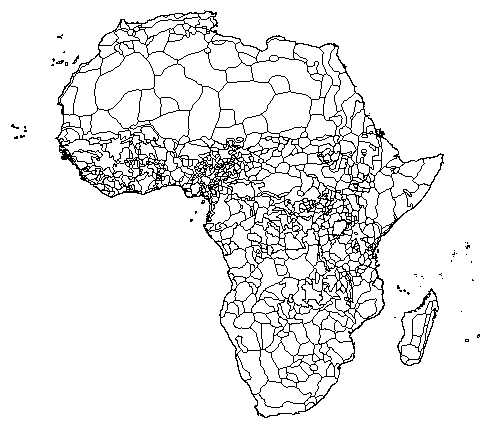
\includegraphics[width=4.8cm]{map murdock.png}
\end{figure}
\end{column}
    
\end{columns}
    \end{itemize}
    \end{frame}

\begin{frame}{Empirical Strategy - Distance on institutional trust (2)}

\begin{itemize}
   \item We limit our sample to individuals living within a 50 km (40km) radius of each side of a border
\end{itemize}

\begin{figure}
    \centering
    \caption{Observations along borders}
    \includegraphics[width=5.5cm]{carte discontinuité (1).png}
\end{figure}

\begin{equation}
trust_{ict}=\beta_{0}+\beta_{1}distance_{ict}+BX_{i}+\textcolor{red}{\mathbf{\nu_{e}}}+\mu_{ct}+\varepsilon_{ict}
\end{equation}

\end{frame}



\begin{frame}{Empirical Strategy - Internet on spatial disparities}

\centering \textbf{Effect of internet use on institutional trust by distance}\vspace{1em}

\begin{itemize}
\item OLS
    \begin{equation}
\begin{split}
trust_{ict} = & \beta_{0} + \beta_{1} distance_{ict} + internet\_use_{ict} + \textcolor{red}{\textbf{distance} \times \textbf{internet\_use}_{ict}} \\
& + BX_{i} + \mu_{ct}+ \varepsilon_{ict}
\end{split}
\end{equation}\vspace{1em}

${internet\_use_{ict}}$ : "how often do you use internet" (values between 0 and 3)\vfill
\item IV
\begin{equation}
\begin{split}
    \textcolor{red}{\textbf{distance} \times \textbf{internet\_use}_{ict}} = & \lambda_{0} + 
    \lambda_{1} \textcolor[rgb]{0.0,0.6,0.0}{\textbf{distance} \times \textbf{internet\_coverage}_{rt}} + BX_{i} \\
    & \quad + \mu_{ct}+ v_{ict}
\end{split}
\end{equation}\\
   $\rightarrow$ Similar to \textit{Guriev et al. (2021)}
\end{itemize}
    
\end{frame}
    
\begin{frame}{Distance increases institutional trust}
    \begin{table}[H]
        \sffamily
        \caption{{Effect of distance to the capital on institutional trust}}
        \centering
        %\footnotesize
        \resizebox{12cm}{!}{
        \begin{tabular}{@{\extracolsep{5pt}} l c c c c c c}
        \\
        \toprule
        \toprule
        &  \multicolumn{6}{c}{{Trust in institutions}}  \\
        \cmidrule(r){2-7}
        & \multicolumn{2}{c}{{OLS}} & \multicolumn{2}{c}{{BDD: 50km}} & \multicolumn{2}{c}{{BDD: 40km}}\\
            \cmidrule(r){2-3}
            \cmidrule(r){4-5}
            \cmidrule(r){6-7}
            & \multicolumn{1}{c}{{(1)}} &  \multicolumn{1}{c}{{(2)}}  & \multicolumn{1}{c}{{(3)}} &  \multicolumn{1}{c}{{(4)}} & \multicolumn{1}{c}{{(5)}} & \multicolumn{1}{c}{(6)}\\
         \midrule
      
         Distance to the capital &       0.224***&       0.322*** & 0.432***&  0.387***& 0.475***&       0.374**\\
         \medskip
         &      (0.03)   &      (0.03)  &  (0.14)   &      (0.14)& (0.14)   &      (0.15)   \\
      
         \midrule
        Standard controls  & Yes & Yes & Yes & Yes& Yes & Yes  \\
        Country X Round FE       & No & Yes& No & Yes& No & Yes\\
        Murdock's area FE & No & No & Yes& Yes& Yes& Yes\\
        Observations      &     83,877   &       83,877  &  18,294   &       18,294 &   16,893   &       16,893\\
        Adjusted-R$^2$        &       0.021   &       0.052  & 0.117   &       0.166 &  0.117   &       0.169  \\
      
                              \bottomrule
        \multicolumn{7}{p{15cm}}{\footnotesize \emph{Notes}: Robust standard errors clustered at the ADM2 x round level  for (1) and (2) and ethnic region for (3-6) are in parentheses. The set of individual controls
        includes values of: normalized distance from the largest non-capital city, age, age squared, sex,
        education, employment status, rural/urban situation, personal economic conditions perception, ADM2 nighttime light.}
        \end{tabular}
        }
        \end{table}
      
\end{frame}

\begin{frame}{Distance increases institutional trust}

\begin{figure}
    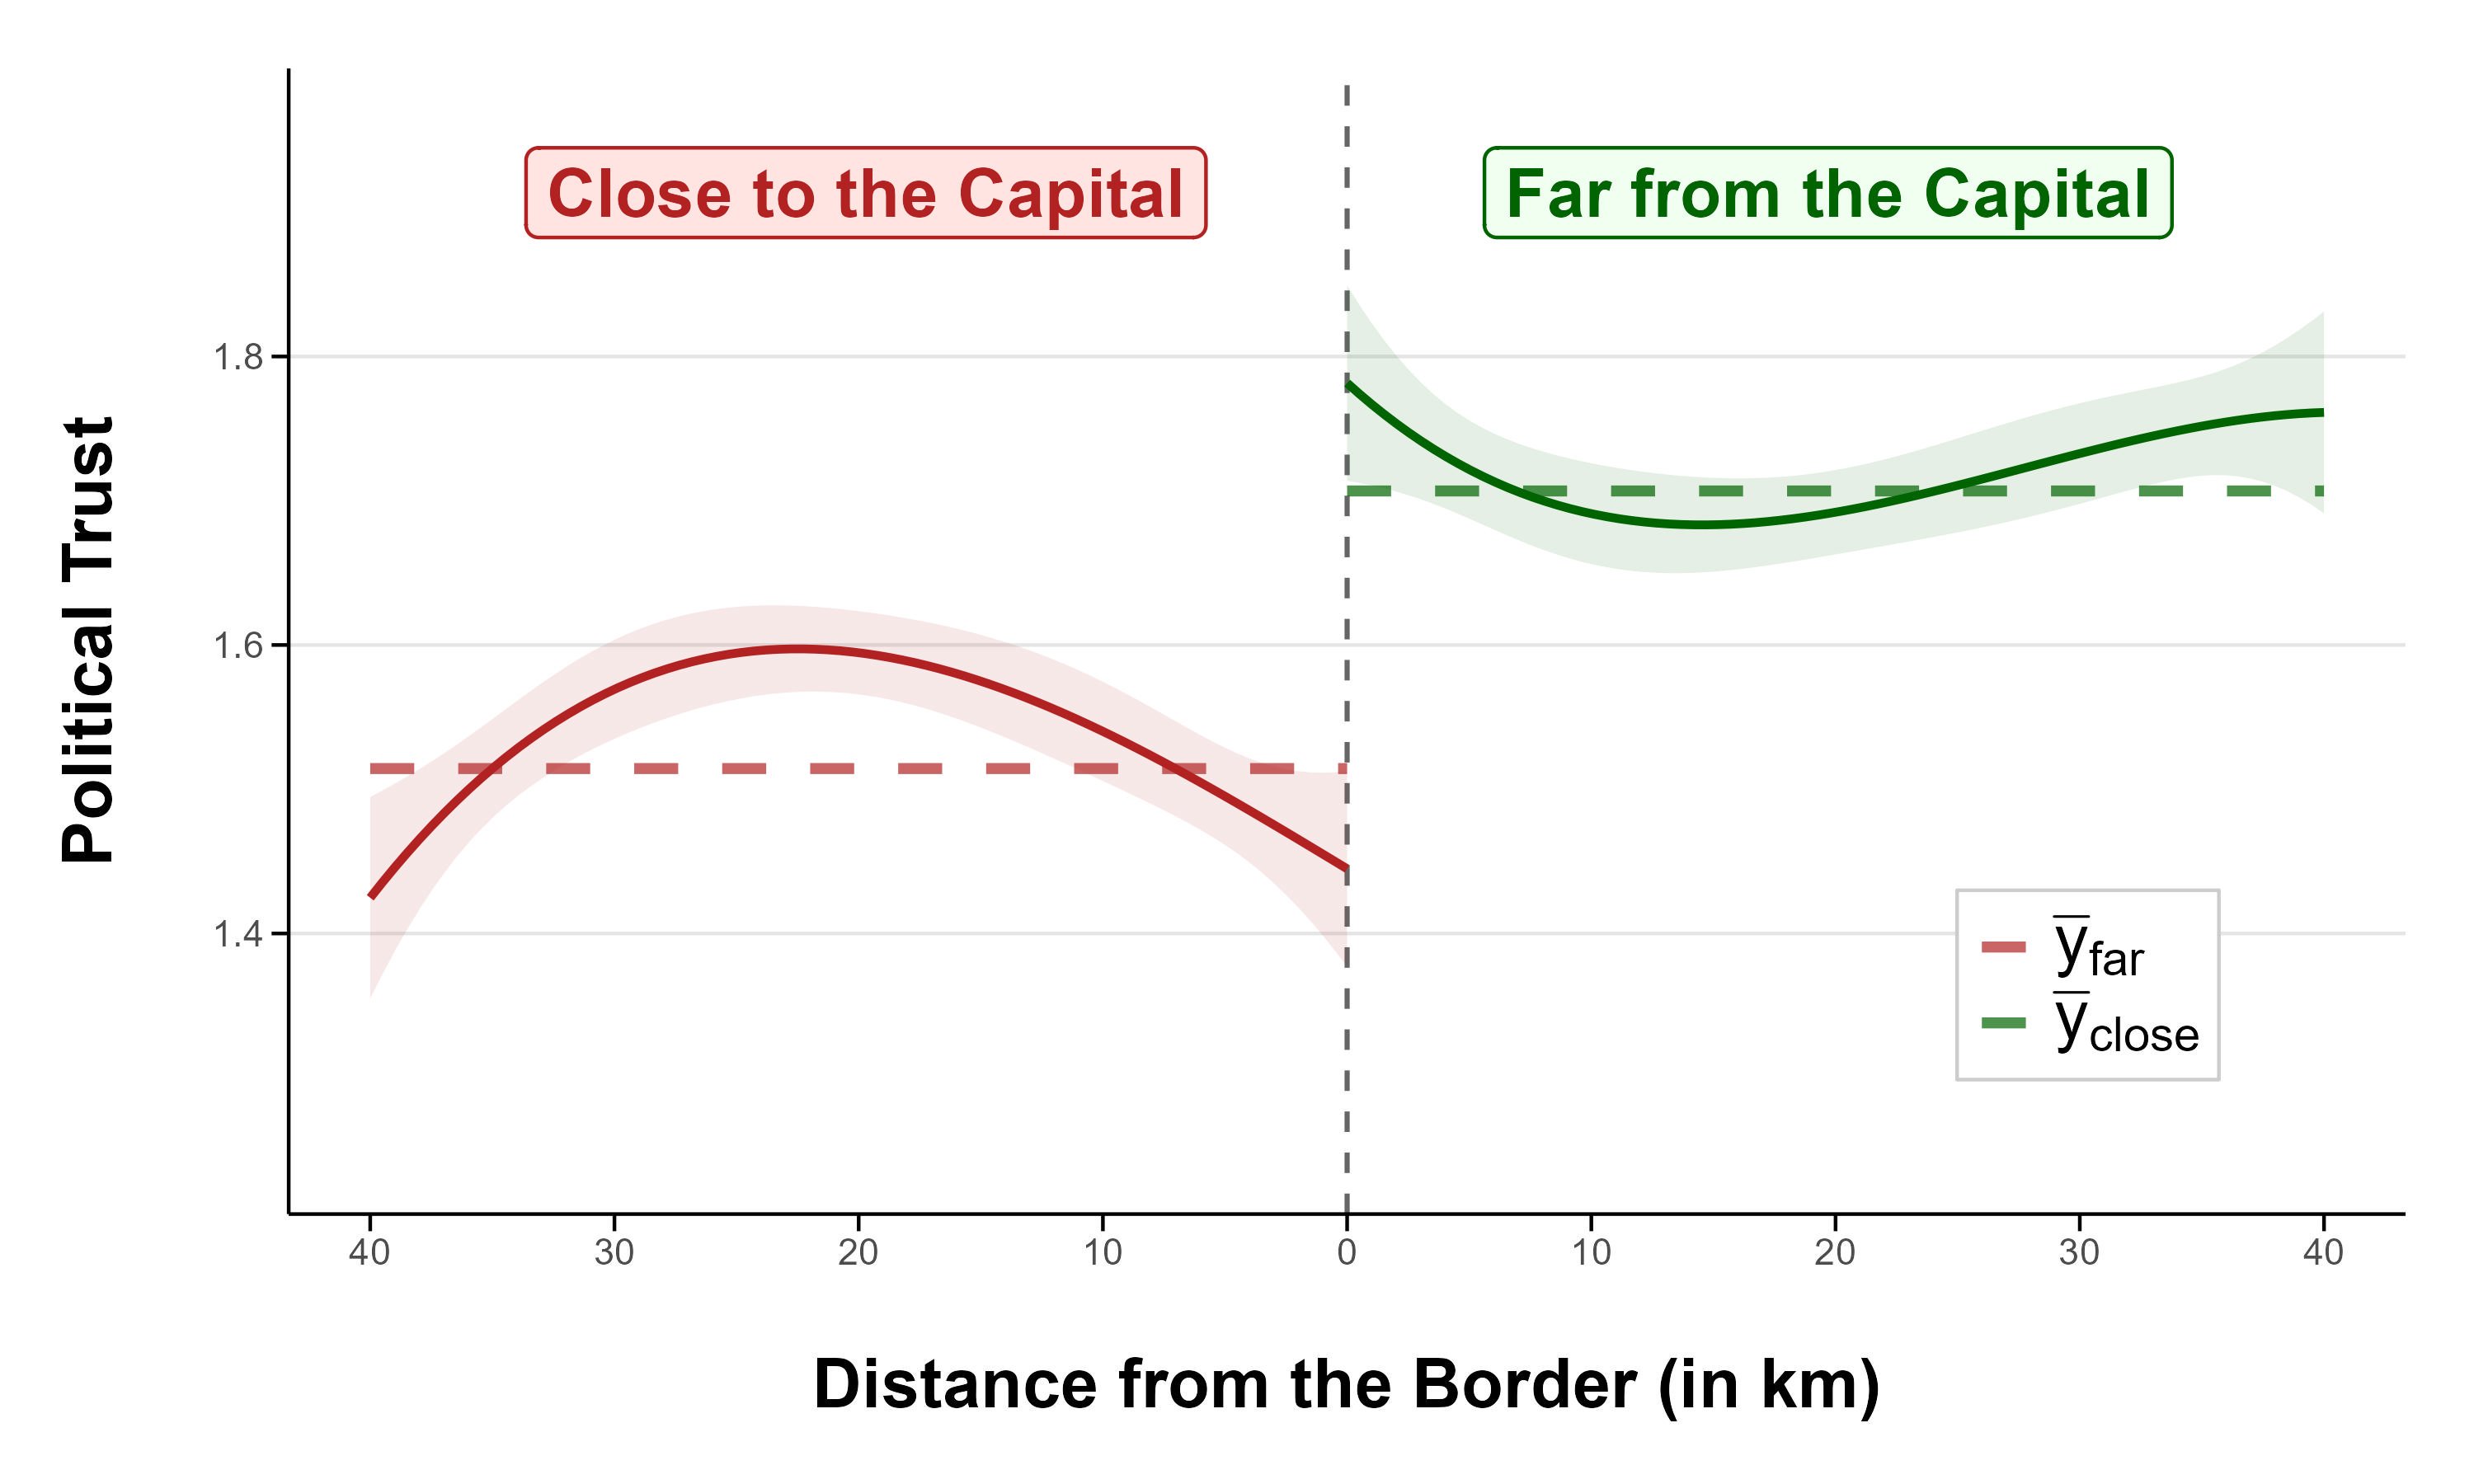
\includegraphics[scale=0.1]{C:/Users/Redha CHABA/Documents/Working paper/Trust/Script/plots/discontinuity/discontinuity.jpg}
    \caption{Border discontinuity - \textit{Based on regression estimates from (4) of Table 1}}
\end{figure}

\end{frame}

\begin{frame}{Internet mitigates spatial disparities}
    \begin{table}[H]
        \sffamily
        \caption{{Effect of internet on institutional trust by distance to the capital}}
        \centering
        %\footnotesize
        \resizebox{12cm}{!}{
        \begin{tabular}{@{\extracolsep{5pt}} l c c c c c c}
        \\
        \toprule
        \toprule
        & \multicolumn{1}{c}{{OLS}} & \multicolumn{3}{c}{{First Stage}} & \multicolumn{1}{c}{{2SLS}}\\
            \cmidrule(r){2-2}
            \cmidrule(r){3-5}
            \cmidrule(r){6-6}
            & \multicolumn{1}{c}{{Trust in institutions}} & \multicolumn{1}{c}{{Internet use}} & \multicolumn{1}{c}{{}} &  \multicolumn{1}{c}{{Distance $\times$ Internet use}} & \multicolumn{1}{c}{{Trust in institutions}}\\
            \cmidrule(r){2-2}
            \cmidrule(r){3-3}
            \cmidrule(r){5-5}
            \cmidrule(r){6-6}
    
            & \multicolumn{1}{c}{{(1)}} & \multicolumn{1}{c}{{(2)}} & \multicolumn{1}{c}{{}} &  \multicolumn{1}{c}{{(3)}} & \multicolumn{1}{c}{{(4)}}\\
            
            \midrule
      
    Distance to the capital&    0.353*** &&&&0.533***\\
         \smallskip
         &      (0.03)  &&&&  (0.117) \\
    Internet use   &      -0.012** &&&&-0.316\\
    \smallskip   &      (0.01)  &&&&  (0.24) \\
    
    Distance to the capital $\times$ Internet use&         -0.054*** &&&&-0.437***\\
    \smallskip  &      (0.01) &&&& (0.14)  \\
    
    
    Internet coverage && 0.179*** && -0.184*** &  &  \\
    \smallskip&& (0.06) && (0.03) \\
    Distance to the capital city $\times$ Internet coverage&& 0.063 && 0.733*** &  & \\
    \medskip&& (0.10) && (0.07)\\
    
         \midrule
        SW \emph{F} - Internet coverage &-&-& 16.12&- &-\\
        SW \emph{F} - Distance $\times$ Internet coverage &-&-& 90.80&-&-\\
        Standard controls  & Yes & Yes &&  Yes & Yes  \\
        Country X Round FE       & Yes & Yes& & Yes & Yes \\
        Observations       &       83,877 & 83,877 & & 83,877 & 83,877 \\
        Adjusted-R$^2$    &       0.164 &  0.358 & &   0.262 & - \\
        %Endogeneity test \emph{p}-value & -& - & - & -& 0.00\\ 
      
                              \bottomrule
        \multicolumn{6}{p{22cm}}{\fontsize{10}{12}\selectfont % Set font size to 8pt with 10pt line spacing
        \emph{Notes}: Robust standard errors clustered at the ADM2 x round level are in parentheses. The set of individual controls
        includes values of: normalized distance from the largest non-capital city, age, age squared, sex,
        education, employment status, rural/urban situation, personal economic conditions perception, ADM2 nighttime light.}
    \end{tabular}}
        \end{table}
    
\end{frame}

\begin{frame}{Internet mitigates spatial disparities}

    
\begin{figure}
    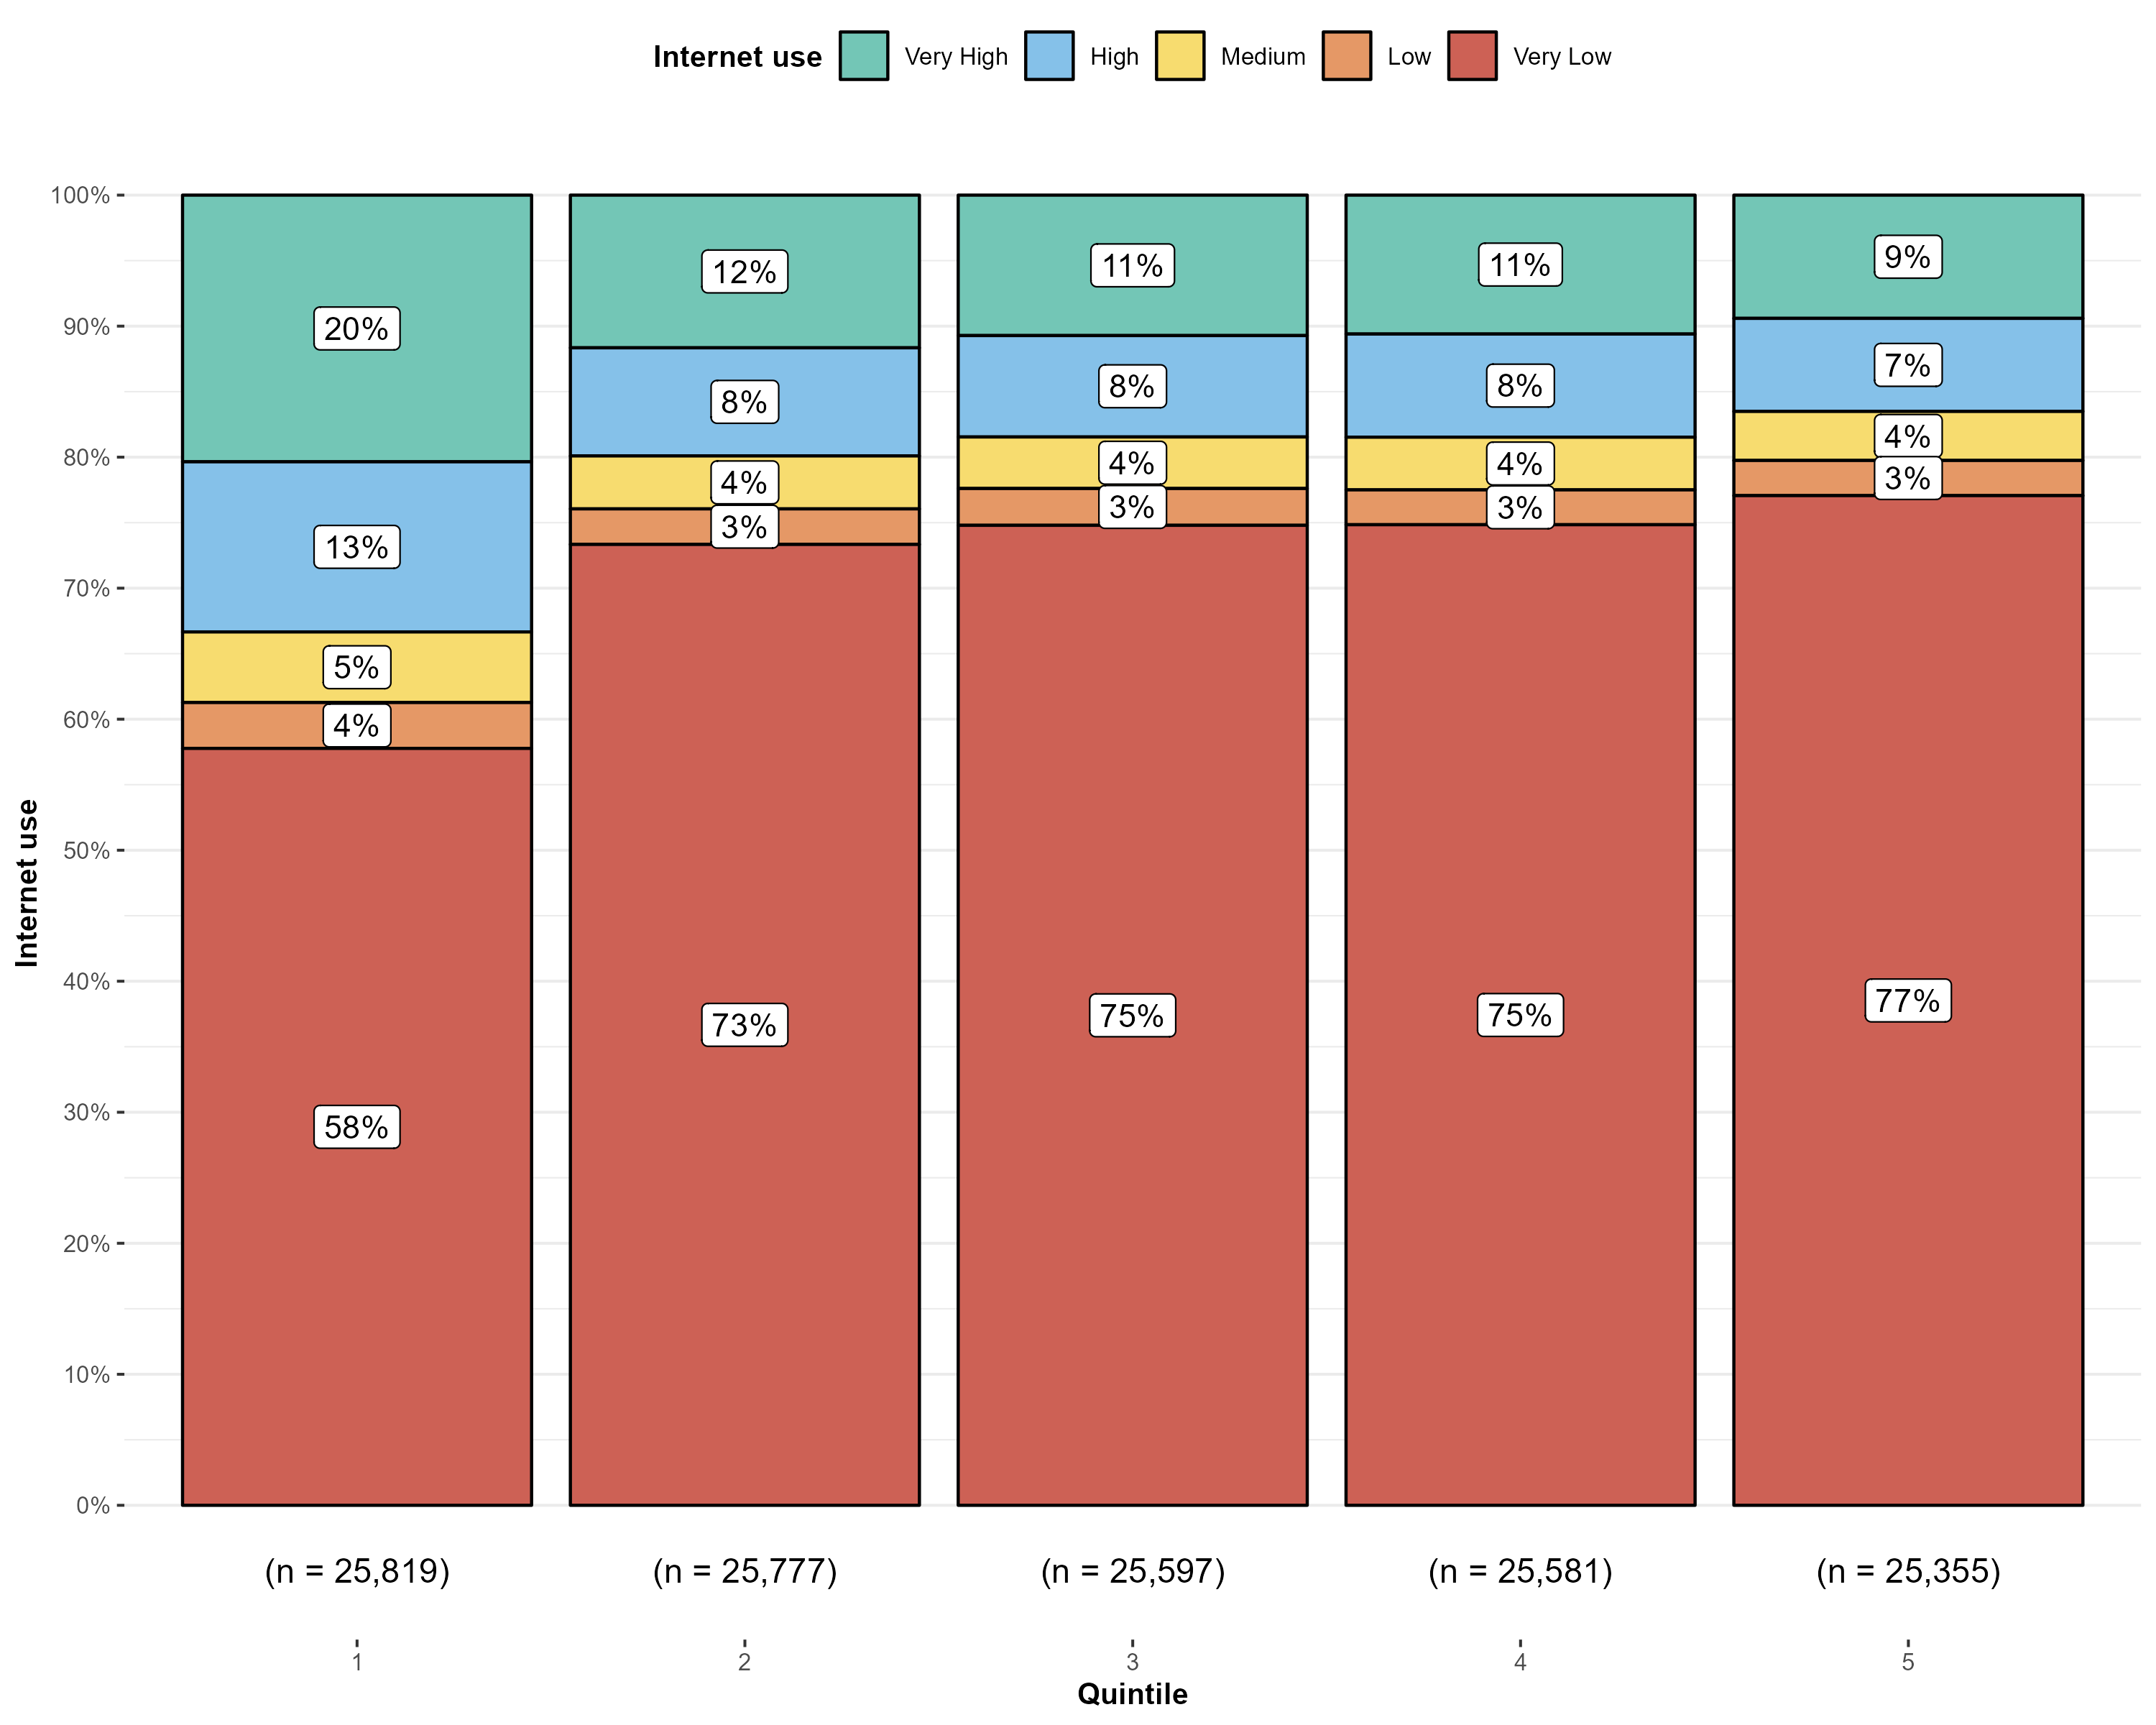
\includegraphics[scale=0.06]{C:/Users/Redha CHABA/Documents/Working paper/Trust/Script/plots/marginal_effect/internet_use.png}
    \caption{Marginal effect of internet use as a function of the distance to the capital}
\end{figure}

\end{frame}



\begin{frame}{Internet mitigates spatial disparities}
 
    \begin{table}[H]
        \sffamily
        \caption{{Effect of internet on national outcomes by distance to the capital}}
        \centering
        %\footnotesize
        \resizebox{12cm}{!}{
        \begin{tabular}{@{\extracolsep{5pt}} l c c c c}
        \\
        \toprule
        \toprule
        & \multicolumn{4}{c}{{2SLS}}\\
        \cmidrule(r){2-5}
        & \multicolumn{3}{c}{{National outcomes}}& \multicolumn{1}{c}{{Placebo}}\\
        \cmidrule(r){2-4}
        \cmidrule(r){5-5}
            & \multicolumn{1}{c}{{Satisfaction in democracy}} & \multicolumn{1}{c}{{Democracy extent}} & \multicolumn{1}{c}{{Trust in ruling party}} & \multicolumn{1}{c}{{Local}} \\
            \cmidrule(r){2-2}
            \cmidrule(r){3-3}
            \cmidrule(r){4-4}
            \cmidrule(r){5-5}
  
    
            & \multicolumn{1}{c}{{(1)}} & \multicolumn{1}{c}{{(2)}} & \multicolumn{1}{c}{{(3)}} & \multicolumn{1}{c}{{(4)}}\\
            
            \midrule
      
    Distance to the capital&  0.316*** & 0.342*** & 0.444***& 0.295***\\
         \smallskip
         & (0.10)& (0.09) & (0.13)&(0.10) \\
    Internet use     & -0.251 & -0.148 & -0.574**& -0.602***\\
    \smallskip      & (0.19) & (0.17)& (0.26)& (0.22)\\
    
    Distance to the capital $\times$ Internet use&   -0.229*  & -0.315***  & -0.356**&  -0.111 \\
    \smallskip & (0.12) & (0.11) & (0.16)& (0.12)\\
    
         \midrule
        Standard controls  & Yes & Yes &Yes&Yes   \\
        Country X Round FE       & Yes & Yes& Yes&Yes  \\
        Observations       &       85,017 & 83,786 & 86,489& 85,953\\
        %Endogeneity test \emph{p}-value & 0.03 & 0.01& 0.00\\ 
      
                              \bottomrule
        \multicolumn{5}{p{21cm}}{\fontsize{10}{12}\selectfont % Set font size to 8pt with 10pt line spacing
        \emph{Notes}: Robust standard errors clustered at the ADM2 x round level are in parentheses. The set of individual controls
        includes values of: normalized distance from the largest non-capital city, age, age squared, sex,
        education, employment status, rural/urban situation, personal economic conditions perception, ADM2 nighttime light.}
    \end{tabular}
        }
        \end{table}
  



\end{frame}

\begin{frame}{Internet enhances corruption perception}

    \begin{table}[H]
        \sffamily
        \caption{{Effect of internet on corruption perception by distance to the capital}}
        \centering
        \resizebox{11cm}{!}{
        \begin{tabular}{@{\extracolsep{5pt}} l c c c c}
        \\
        \toprule
        \toprule
        & \multicolumn{4}{c}{{2SLS}}\\
        \cmidrule(r){2-5}
        & \multicolumn{3}{c}{{National outcomes}}& \multicolumn{1}{c}{{Placebo}}\\
        \cmidrule(r){2-4}
        \cmidrule(r){5-5}
            & \multicolumn{1}{c}{{President}} & \multicolumn{1}{c}{{Parliament}} & \multicolumn{1}{c}{{Judiciary}} & \multicolumn{1}{c}{{Local}} \\
            \cmidrule(r){2-2}
            \cmidrule(r){3-3}
            \cmidrule(r){4-4}
            \cmidrule(r){5-5}
  
    
            & \multicolumn{1}{c}{{(1)}} & \multicolumn{1}{c}{{(2)}} & \multicolumn{1}{c}{{(3)}}& \multicolumn{1}{c}{{(4)}}\\
            
            \midrule
      
    Distance to the capital& -0.286***  & -0.302***  & -0.296*** &    -0.202** \\
         \smallskip
         & (0.09)& (0.08) & (0.08) & (0.08) \\
    Internet use   & 0.242 & 0.057  & 0.089&   0.160\\
    \smallskip  & (0.17) & (0.15)& (0.17)& (0.16)  \\
    
    Distance to the capital $\times$ Internet use& 0.277***   & 0.321***   & 0.336*** &   0.129  \\
    \smallskip  & (0.10) & (0.09) & (0.10)  & (0.09)\\
    
         \midrule
        Standard controls  & Yes & Yes &Yes& Yes  \\
        Country X Round FE       & Yes & Yes& Yes& Yes \\
        Observations       &       80,370& 81,590 & 81,705 &  79,545  \\
        %Endogeneity test \emph{p}-value & 0.01 & 0.00 & 0.00\\ 
      
                              \bottomrule
        \multicolumn{5}{p{14cm}}{\fontsize{9}{11}\selectfont % Set font size to 8pt with 10pt line spacing
        \emph{Notes}: Robust standard errors clustered at the ADM2 x round level are in parentheses. The set of individual controls
        includes values of: normalized distance from the largest non-capital city, age, age squared, sex,
        education, employment status, rural/urban situation, personal economic conditions perception, ADM2 nighttime light.}
    \end{tabular}}
        \end{table}
\end{frame}

\begin{frame}{Stronger effects in autocratic and media-captured countries}
    \begin{table}[H]
        \sffamily
        \caption{{Variations by institution and media freedom}}
        \centering
        %\footnotesize
        \resizebox{11cm}{!}{
        \begin{tabular}{@{\extracolsep{5pt}} l c c c c}
        \\
        \toprule
        \toprule
        & \multicolumn{4}{c}{{2SLS}}\\
            \cmidrule(r){2-5}
            & \multicolumn{2}{c}{{Institutions}} & \multicolumn{2}{c}{{Medias}} \\
            \cmidrule(r){2-3}
            \cmidrule(r){4-5}
            & \multicolumn{1}{c}{{Democratic}} & \multicolumn{1}{c}{{Autocratic}}& \multicolumn{1}{c}{{Free}} & \multicolumn{1}{c}{{Captured}} \\
            \cmidrule(r){2-2}
            \cmidrule(r){3-3}
            \cmidrule(r){4-4}
            \cmidrule(r){5-5}

          
            & \multicolumn{1}{c}{{(1)}} & \multicolumn{1}{c}{{(2)}} & \multicolumn{1}{c}{{(3)}} & \multicolumn{1}{c}{{(4)}}\\
            
            \midrule
      
    Distance to the capital& 0.363 & 0.683*** & 0.364** & 0.719***\\
         \smallskip
         & (0.25)   & (0.15) & (0.17)  & (0.13)   \\
    Internet use & -0.643 & -0.065  & -0.498* & 0.080\\
    \smallskip    & (0.48) & (0.31) & (0.27)& (0.27) \\
    
    Distance to the capital $\times$ Internet use & -0.217 & -0.638*** & -0.303 & -0.581*** \\
    \smallskip & (0.28) & (0.20)& (0.22) & (0.17) \\
    
         \midrule
        Standard controls  & Yes & Yes& Yes & Yes\\
        Country X Round FE & Yes & Yes & Yes & Yes\\
        Observations  & 44,434  & 39,443  & 36,872  & 47,005   \\
        %Endogeneity test \emph{p}-value & 0.00 & 0.03 & 0.04 & 0.00 \\ 
      
                              \bottomrule
        \multicolumn{5}{p{14cm}}{\fontsize{8}{11}\selectfont % Set font size to 8pt with 10pt line spacing
        \emph{Notes}: Robust standard errors clustered at the ADM2 x round level are in parentheses. The set of individual controls
        includes values of: normalized distance from the largest non-capital city, age, age squared, sex,
        education, employment status, rural/urban situation, personal economic conditions perception, ADM2 nighttime light.}
    \end{tabular}}
        \end{table}
\end{frame}

\begin{frame}{Upcoming research}

    \begin{itemize}
        \item Explore another result:\vspace{0.5em}
        \begin{itemize}
            \item National identification, vote, voter turnout\vspace{0.5em}
            \item Variations in duration of internet exposure\vspace{0.5em}
        \end{itemize}
        \item Explore the role of social medias\vspace{0.5em}
        \item Heterorogeneity: regime type, Sub-Saharan African regions, colonial legacy
    \end{itemize}
    
\end{frame}

\end{document}